\appendix

\clearpage\section{Detailed electrical system}
The voltage drop over a series shunt resistor is measured using a differential amplifier. This voltage drop, which is linearly proportional to to the current that flows through the quartz crystal as described by Ohm's law, is indicative of the changing impedance of the crystal as a function of frequency. Therefore, this signal can be used to show when the crystal is on resonance. 

A more detailed schematic can be found in \autoref{fig:detsch}. Preliminary tests showed that the peak voltage of about $V_{p}=10$~V is needed to see a significant amplitude-frequency dependence. The maximum current at this voltage is about $I_{p}=200$~mA. A high speed operational amplifier was used in combination with a buffer amplifier in the feedback path to decrease the output impedance and increase the output current capability of the amplifier. The slew rate of the amplifier is also an important parameter, since the signal has both high frequency and high amplitude. The needed slew rate corresponds to the maximum slope of the output signal, which for a sinusoidal signal of the following form:
\begin{equation}\label{eq:driving}
v(t) = V_{P} \sin{2\pi ft},
\end{equation}
is given by:
\begin{equation}\label{eq:slewrate}
\mbox{max}\left(\left|\frac{dv(t)}{dt}\right|\right) = \frac{\pi fV_{P}}{2}.
\end{equation}
Using crystal frequency of $f=\SI{4.606}{\mega\hertz}$ and a peak voltage of $V_{p}=10$~V, the minimum slew rate of the amplifier should therefore be \SI{425}{\volt/\micro\second}. 

\begin{figure}
	\centering
		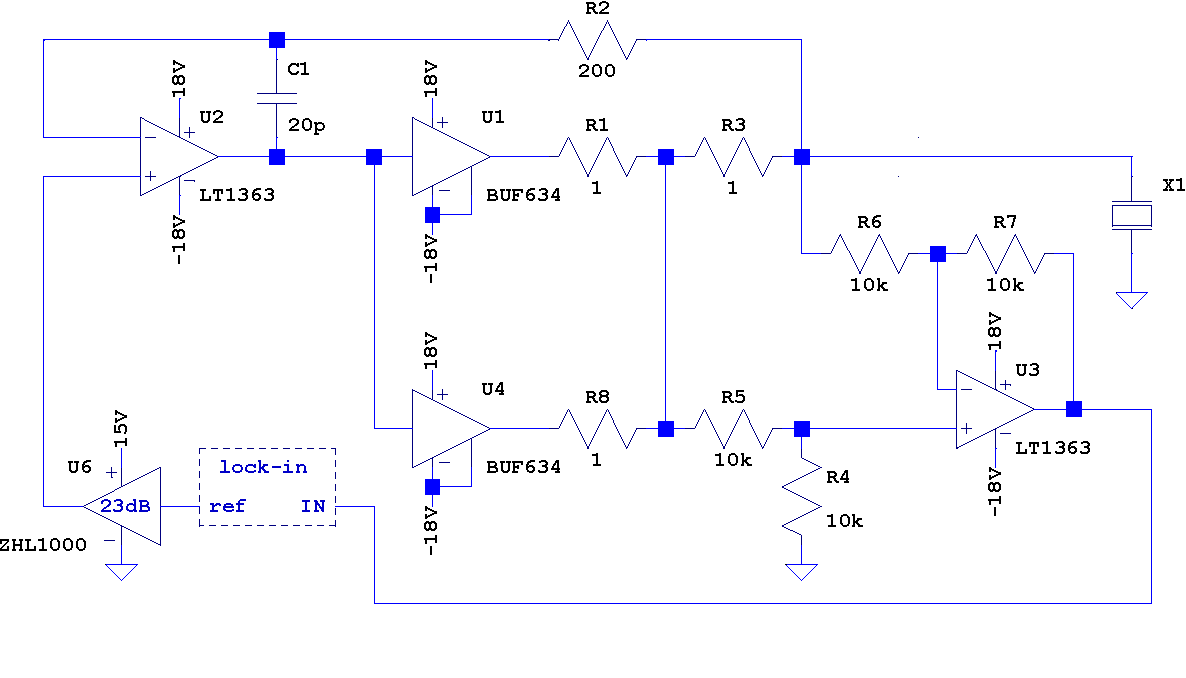
\includegraphics[width=\textwidth]{figures/BUF634_paper.pdf}
	\caption{Detailed schematic of the electrical system of the experimental set-up. }
	\label{fig:detsch}
\end{figure}


\clearpage\section{Temperature-based quartz crystal relaxation oscillator}